\subsection{Übersichtszeichnung}

\begin{figure}[h!]
	\centering
	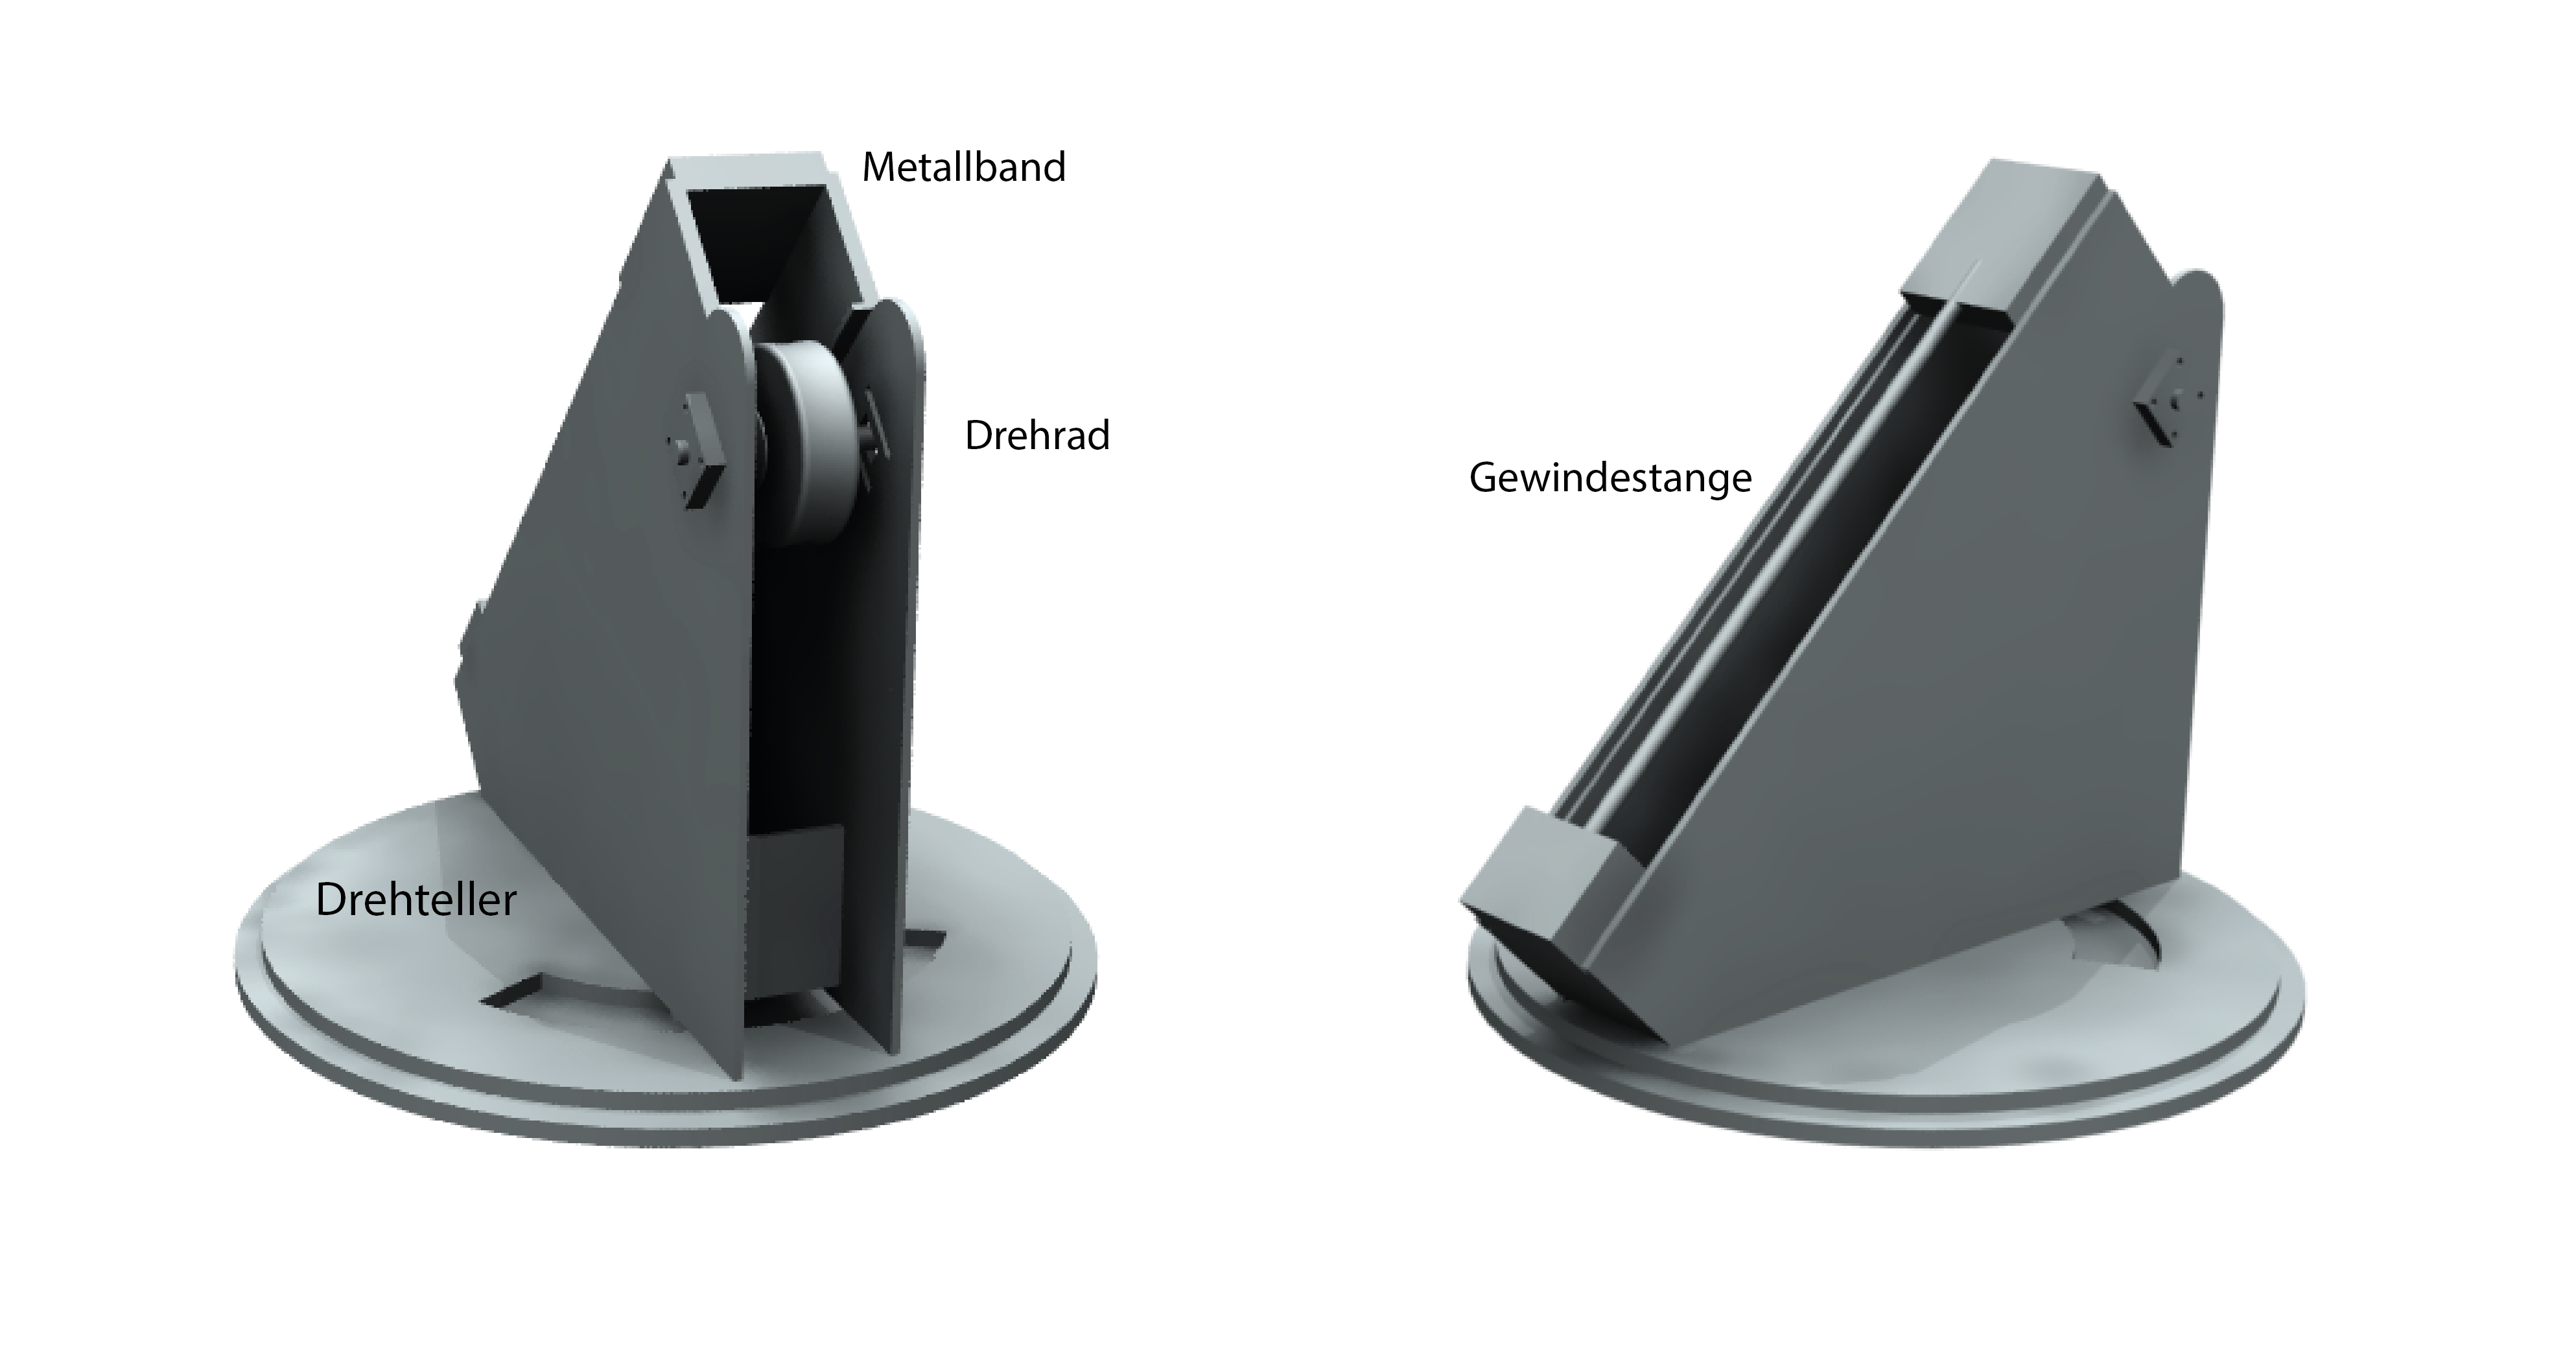
\includegraphics[scale=0.5]{../../fig/StudioLegende.png}
	\caption{Gesamtkonstruktion}
\end{figure}

Für die Realisierung der Wurfmaschine ist ein Aufbau mittels zwei senkrecht stehenden Hauptplatten vorgesehen, welche aus Holz oder Kunststoff bestehen. Zu Grunde der Platten liegt der Drehteller. Alle Bauteile werden zwischen diesen beiden Hauptplatten untergebracht.

\newpage

\begin{figure}[h!]
	\centering
	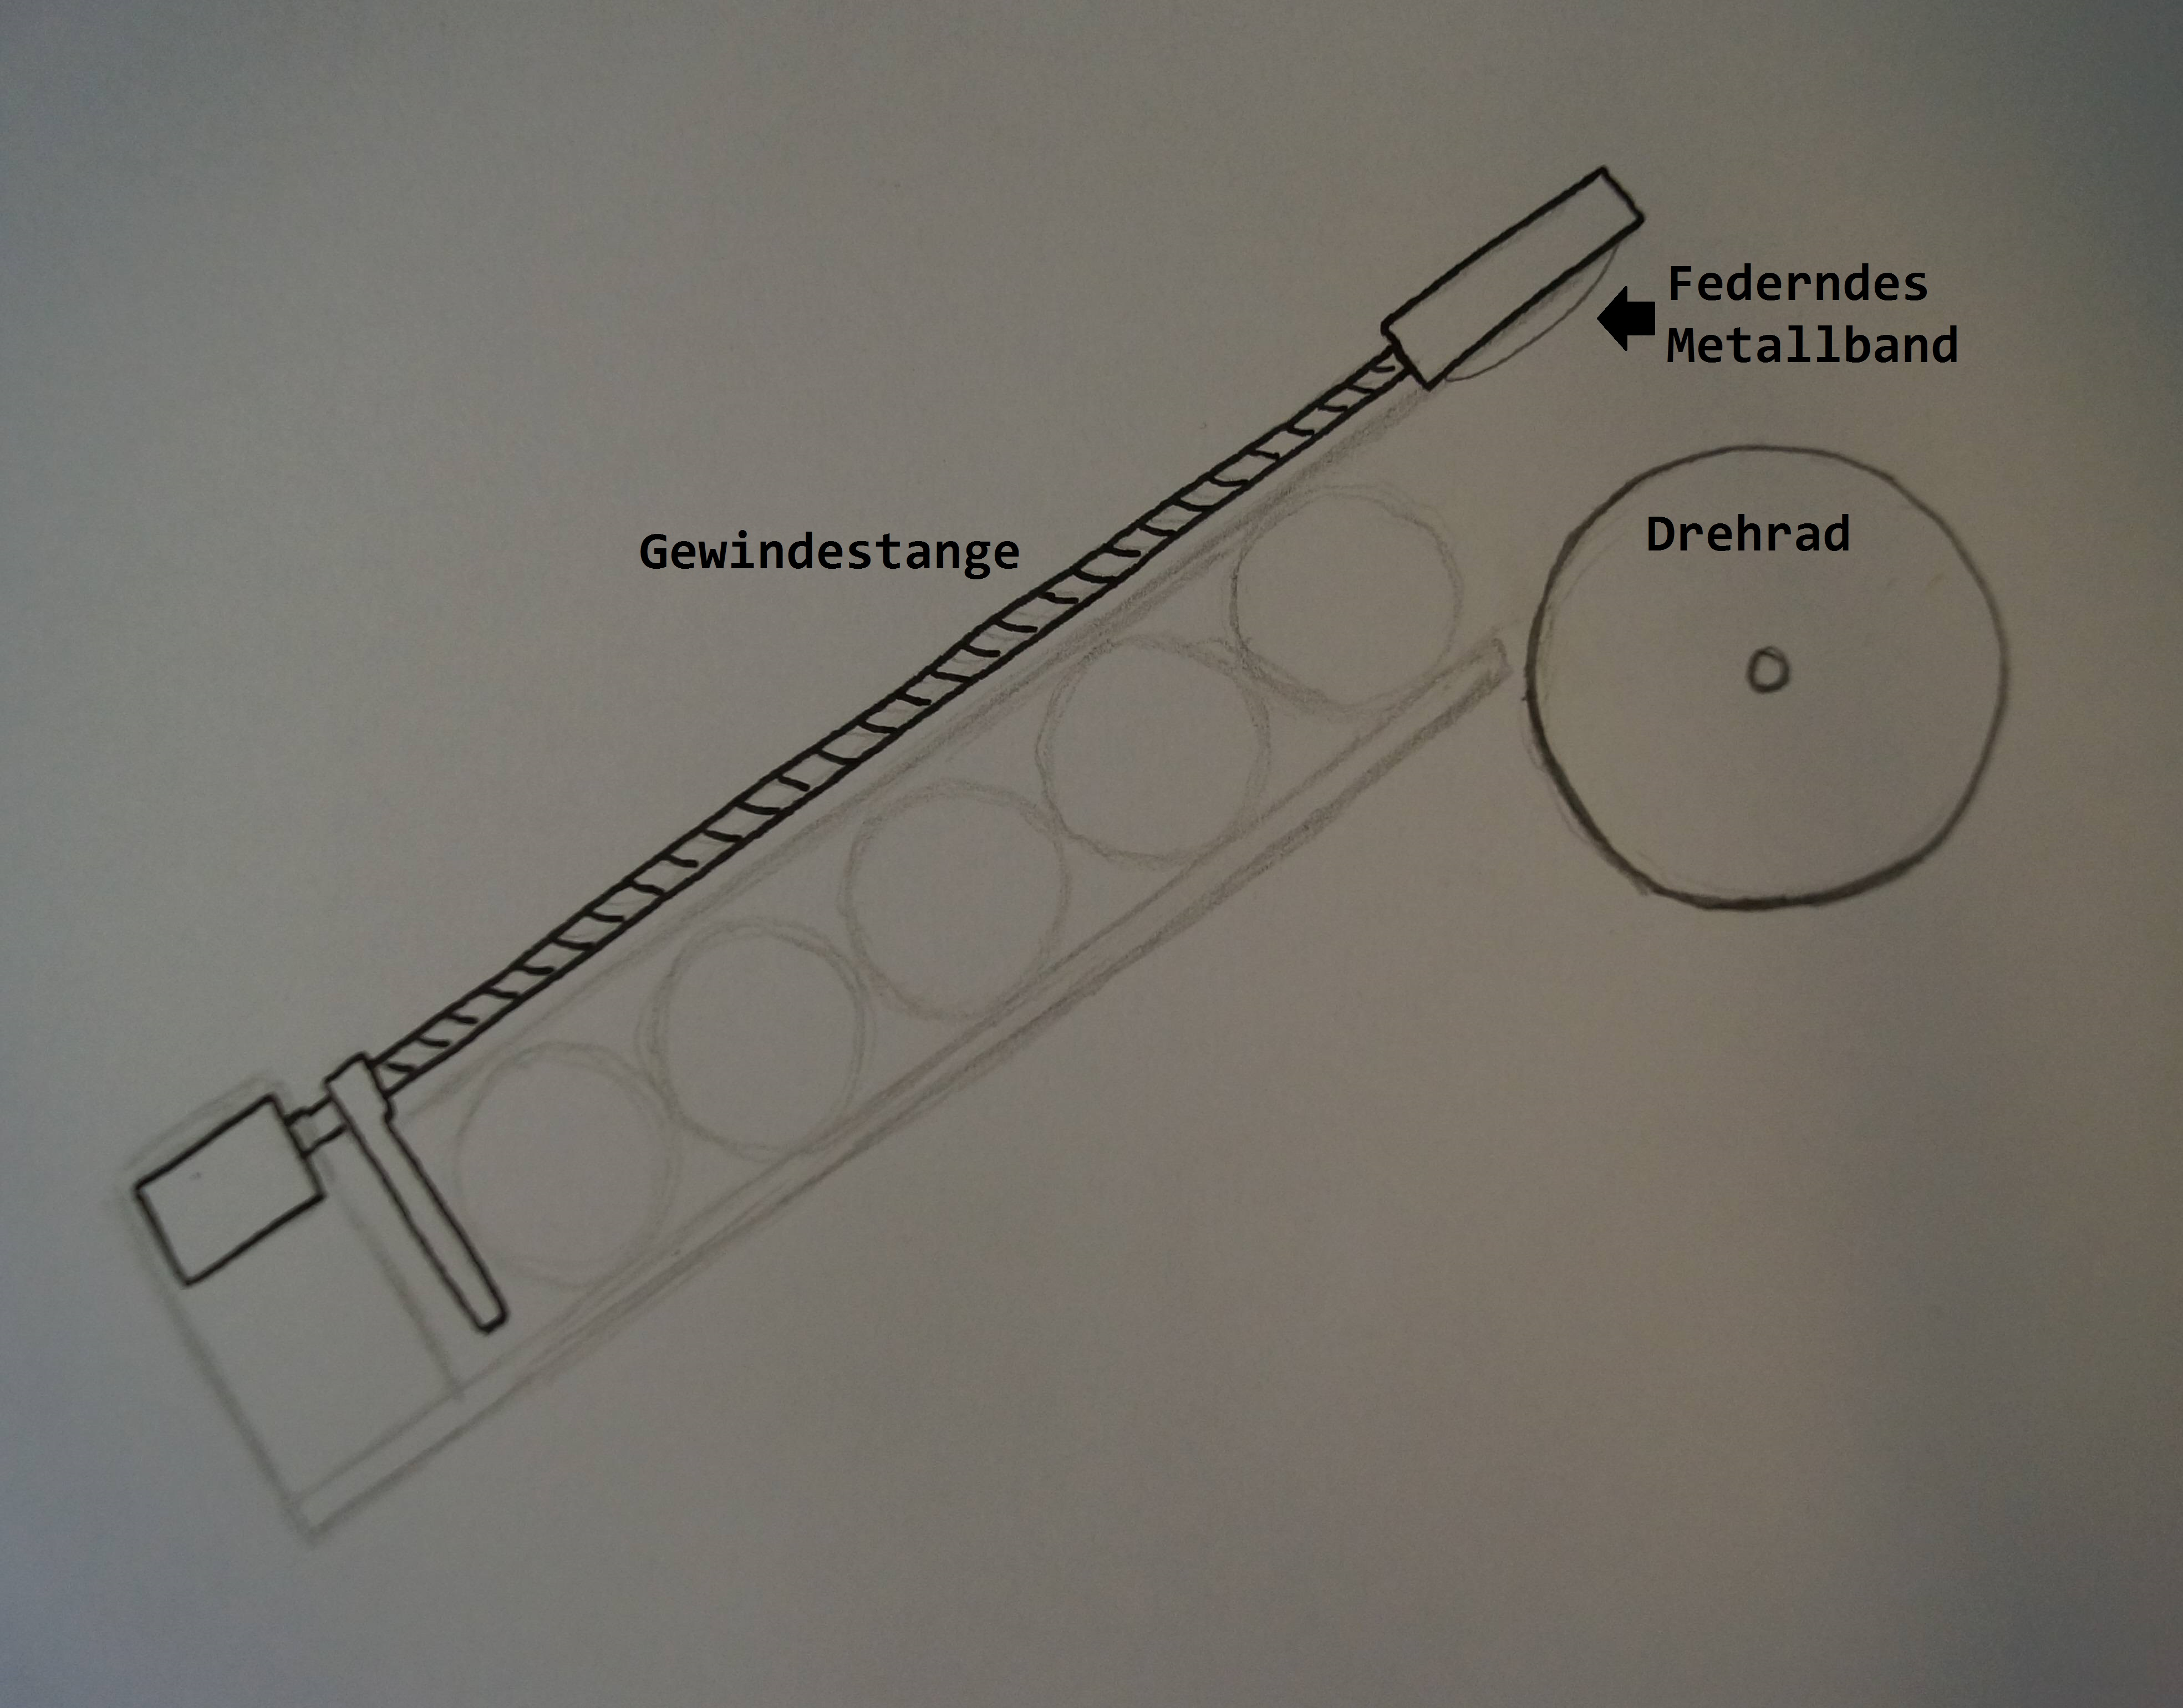
\includegraphics[scale=0.35]{../../fig/Ballnachlader.jpg}
	\caption{Nachlade-Mechanismus}
	\label{fig:nachlade-machanismus}
\end{figure}

Wie in Abbildung \ref{fig:nachlade-machanismus} zu sehen ist, wird der Ballnachschub mit einer Gewindestange realisiert. Die Gewindestange wird durch einen direkt angebundenen Motor in Rotation gebracht. Dadurch bringt die Gewindestange einen Mitnehmer in eine Linearbewegung entlang der Stangenachse und bewegt dadurch die Tennisbälle in Richtung Drehrad.

\begin{figure}[h!]
	\centering
	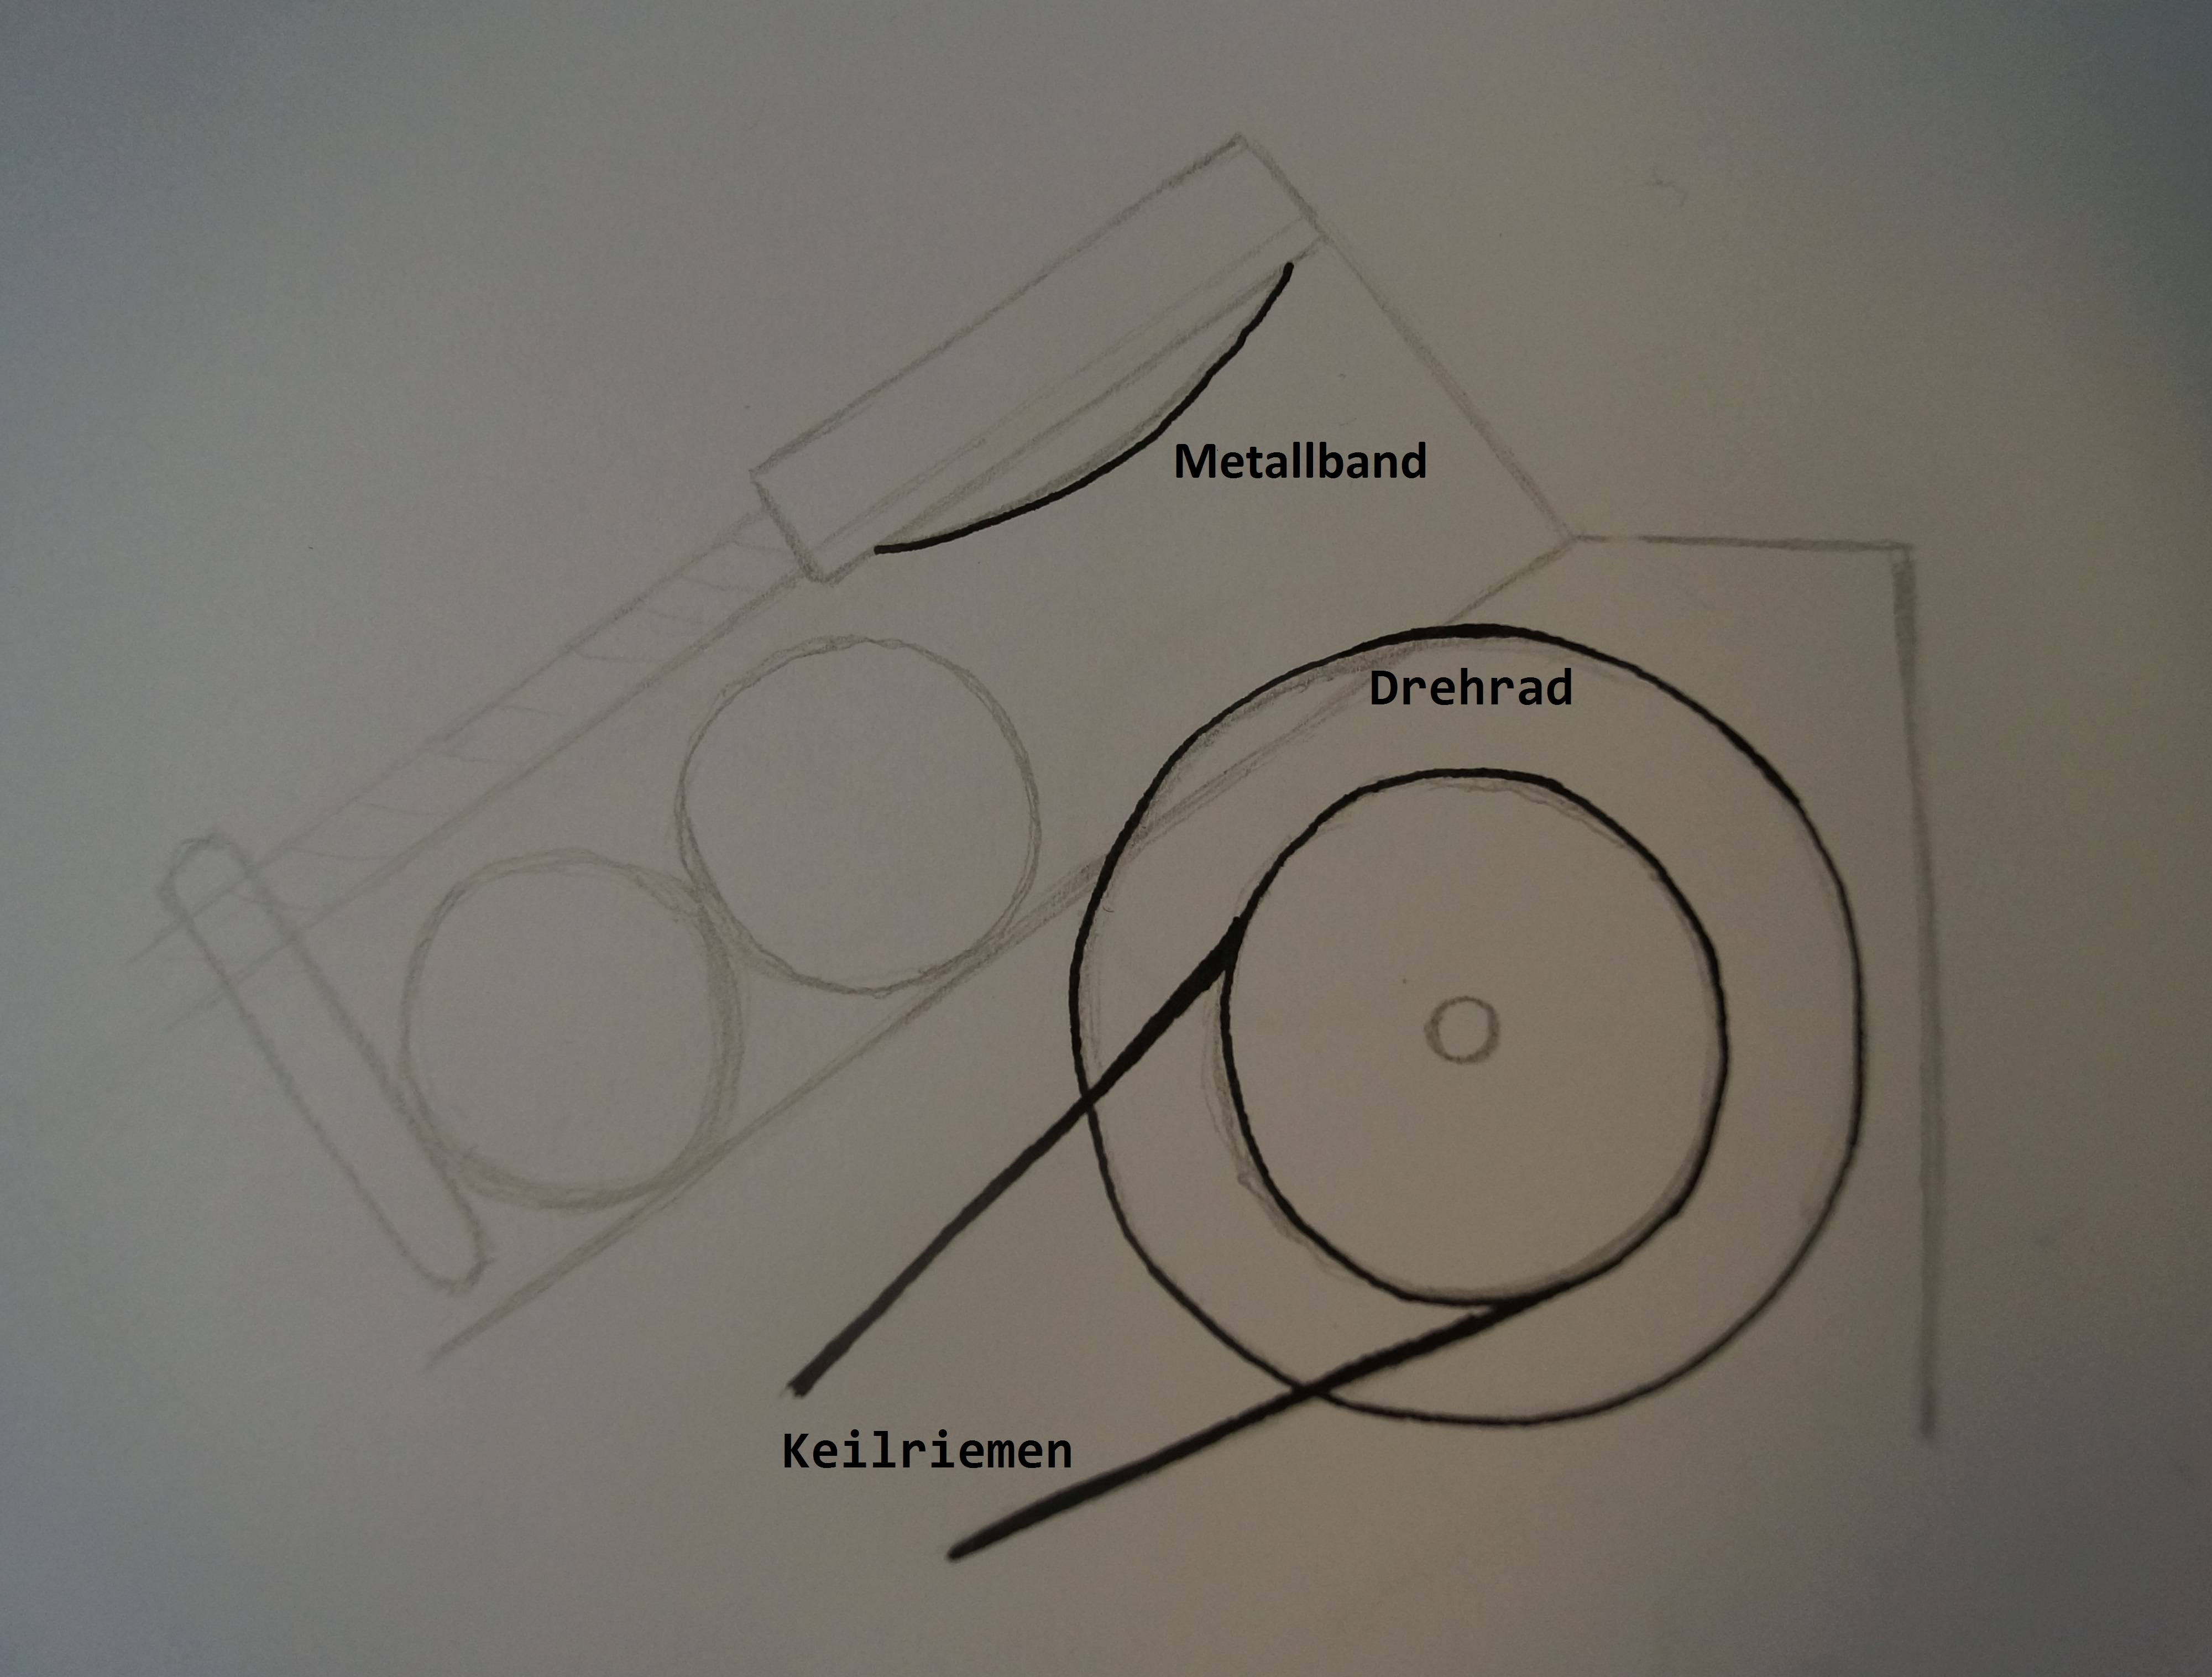
\includegraphics[scale=0.35]{../../fig/Drehrad.jpg}
	\caption{Aufbau des Drehrades}
\end{figure}

Die Bälle werden durch ein rotierendes Drehrad beschleunigt. Das Drehrad wiederum erhält seine Rotation durch einen angebauten Keilriemen (oder Zahnriemen), welcher mit einem Motor verbunden ist. Um mögliche Grössenunterschiede der Bälle kompensieren zu können, kommt ein Metallband zum Zug, welches über dem Rad angebracht ist.

\newpage

\begin{figure}[h!]
	\centering
	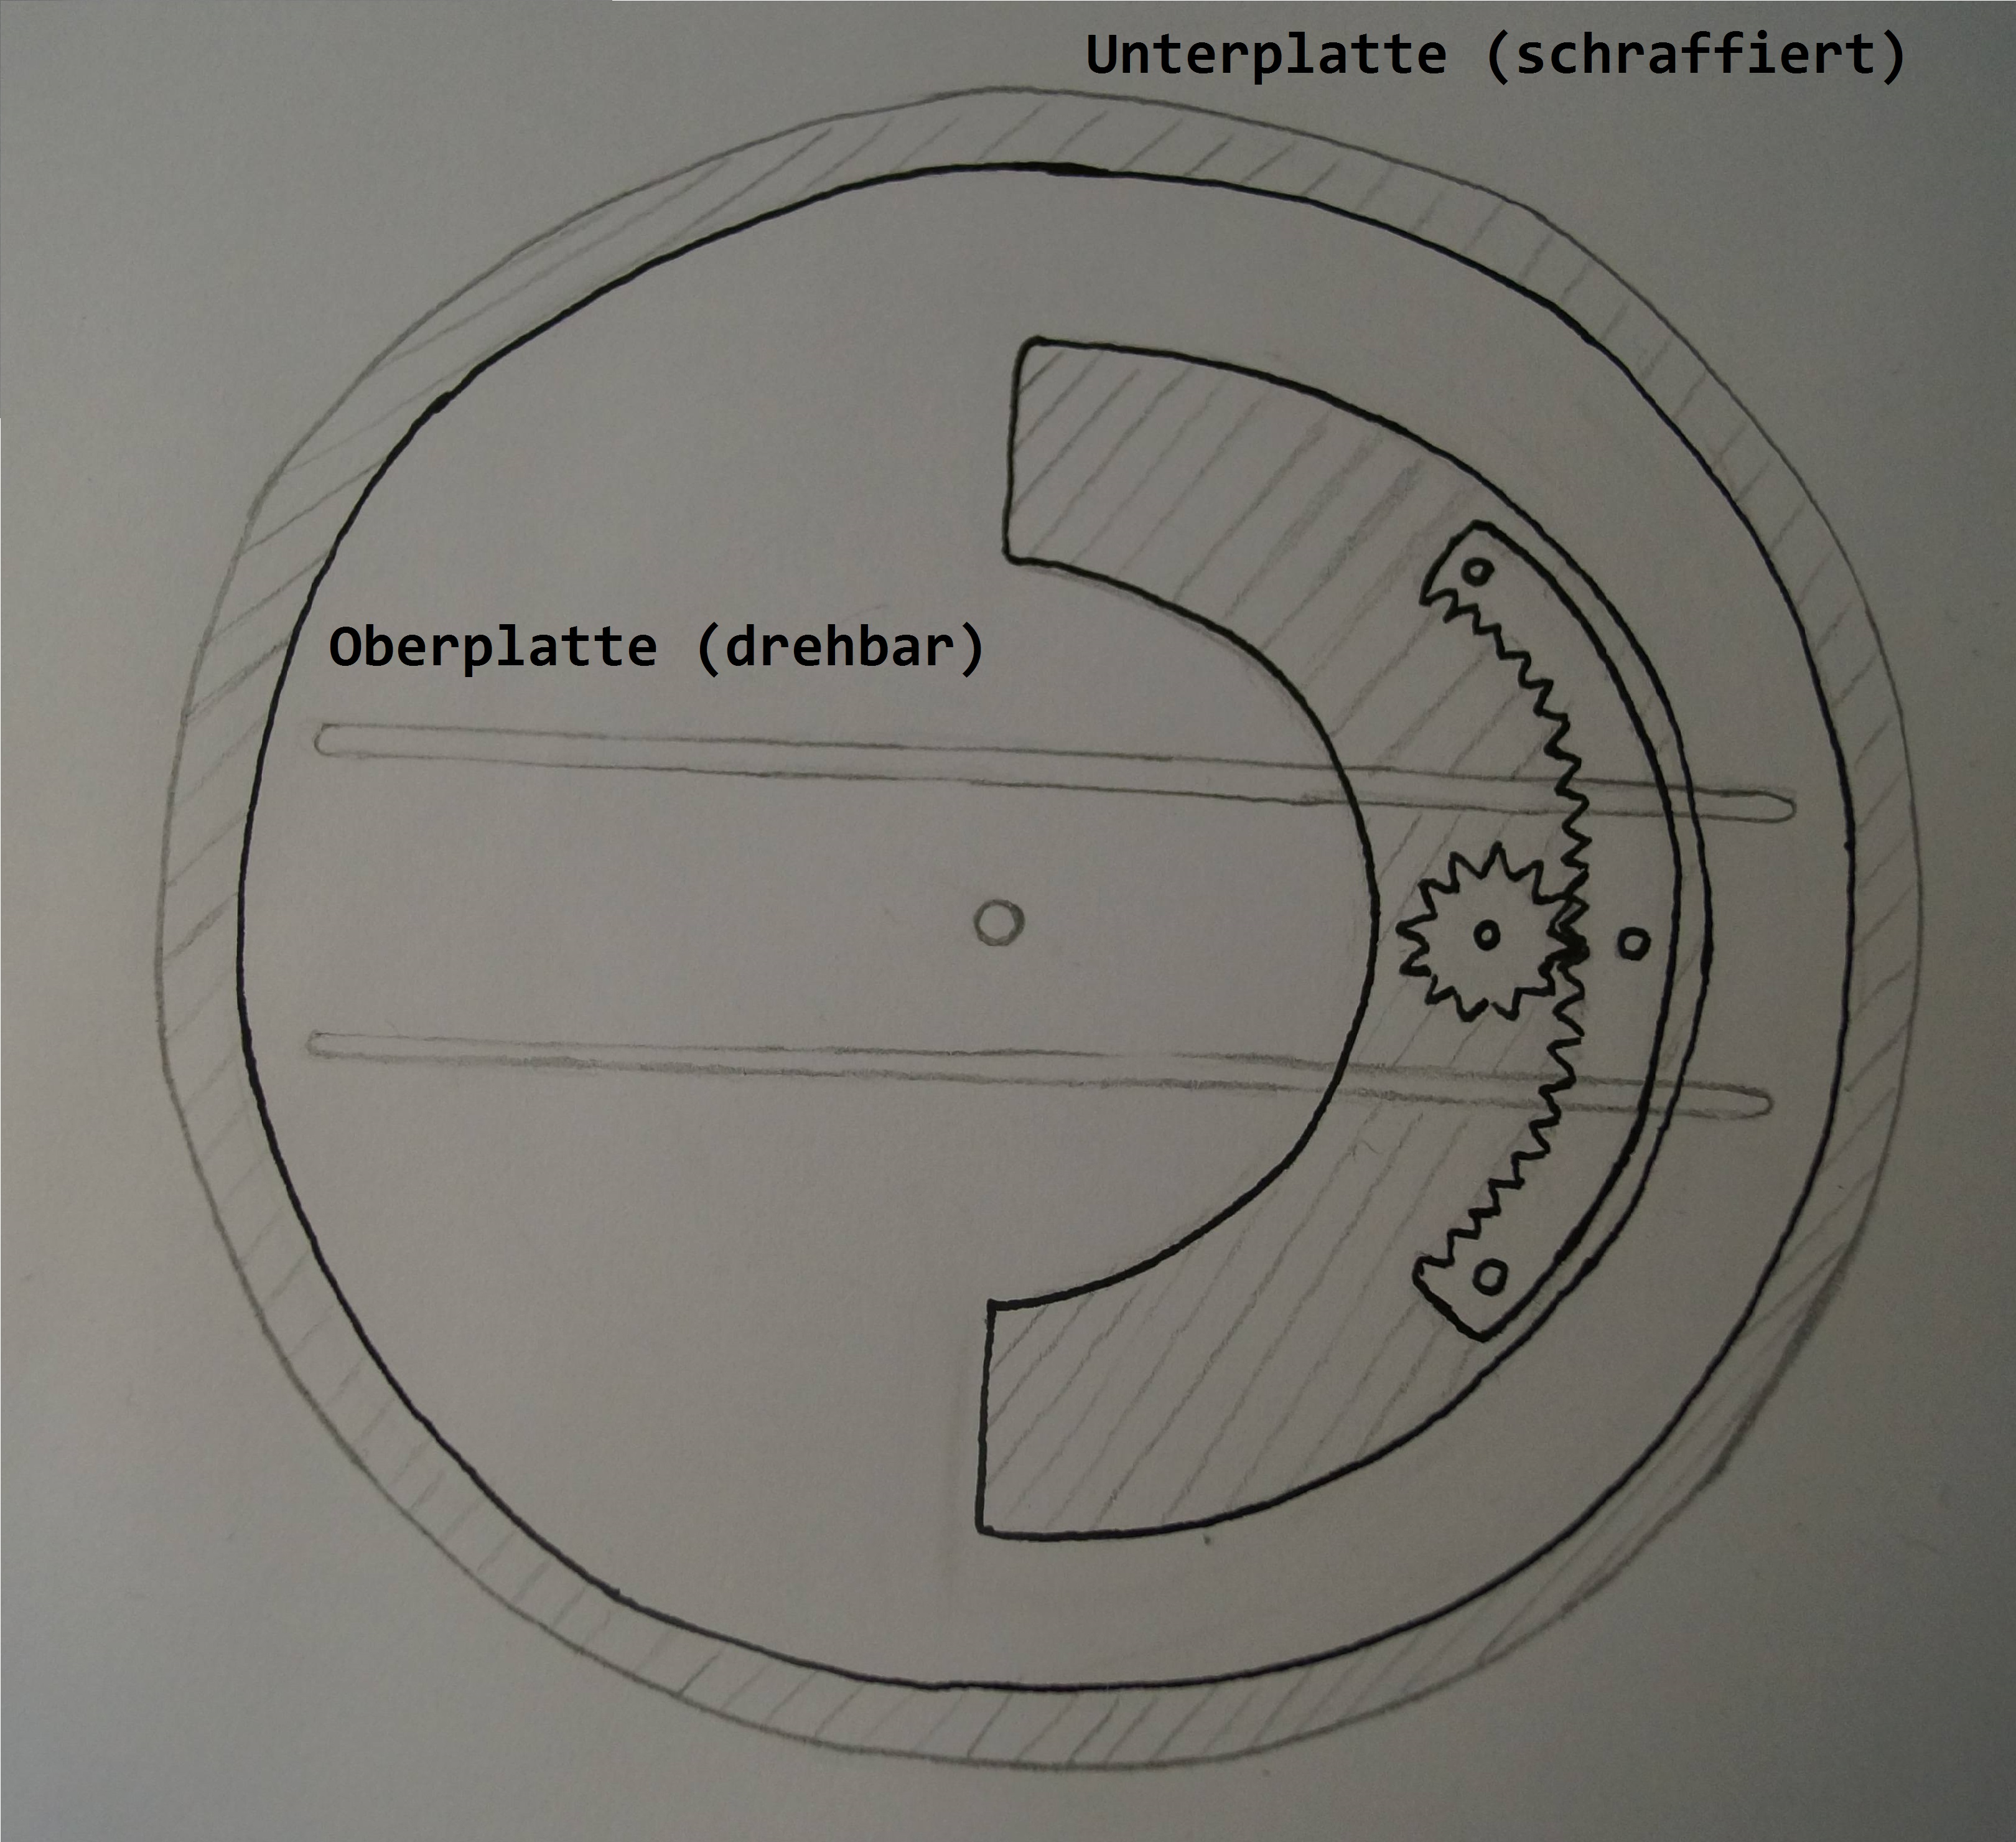
\includegraphics[scale=0.35]{../../fig/Ausrichtvorrichtung_Oben.jpg}
	\caption{Ausricht-Vorrichtung von oben}
\end{figure}

Um die Wurfmaschine horizontal auf den Korb auszurichten, wird die ganze Abschussvorrichtung auf einem Drehteller montiert, welcher auf einer Grundplatte gelagert liegt. An einer auf der Grundplatte befestigten Zahnscheibe, kann nun ein am Drehteller montiertes, angetriebenes Zahnrad, durch Eingriff an der Zahnscheibe, den Drehteller drehen.

\begin{figure}[h!]
	\centering
	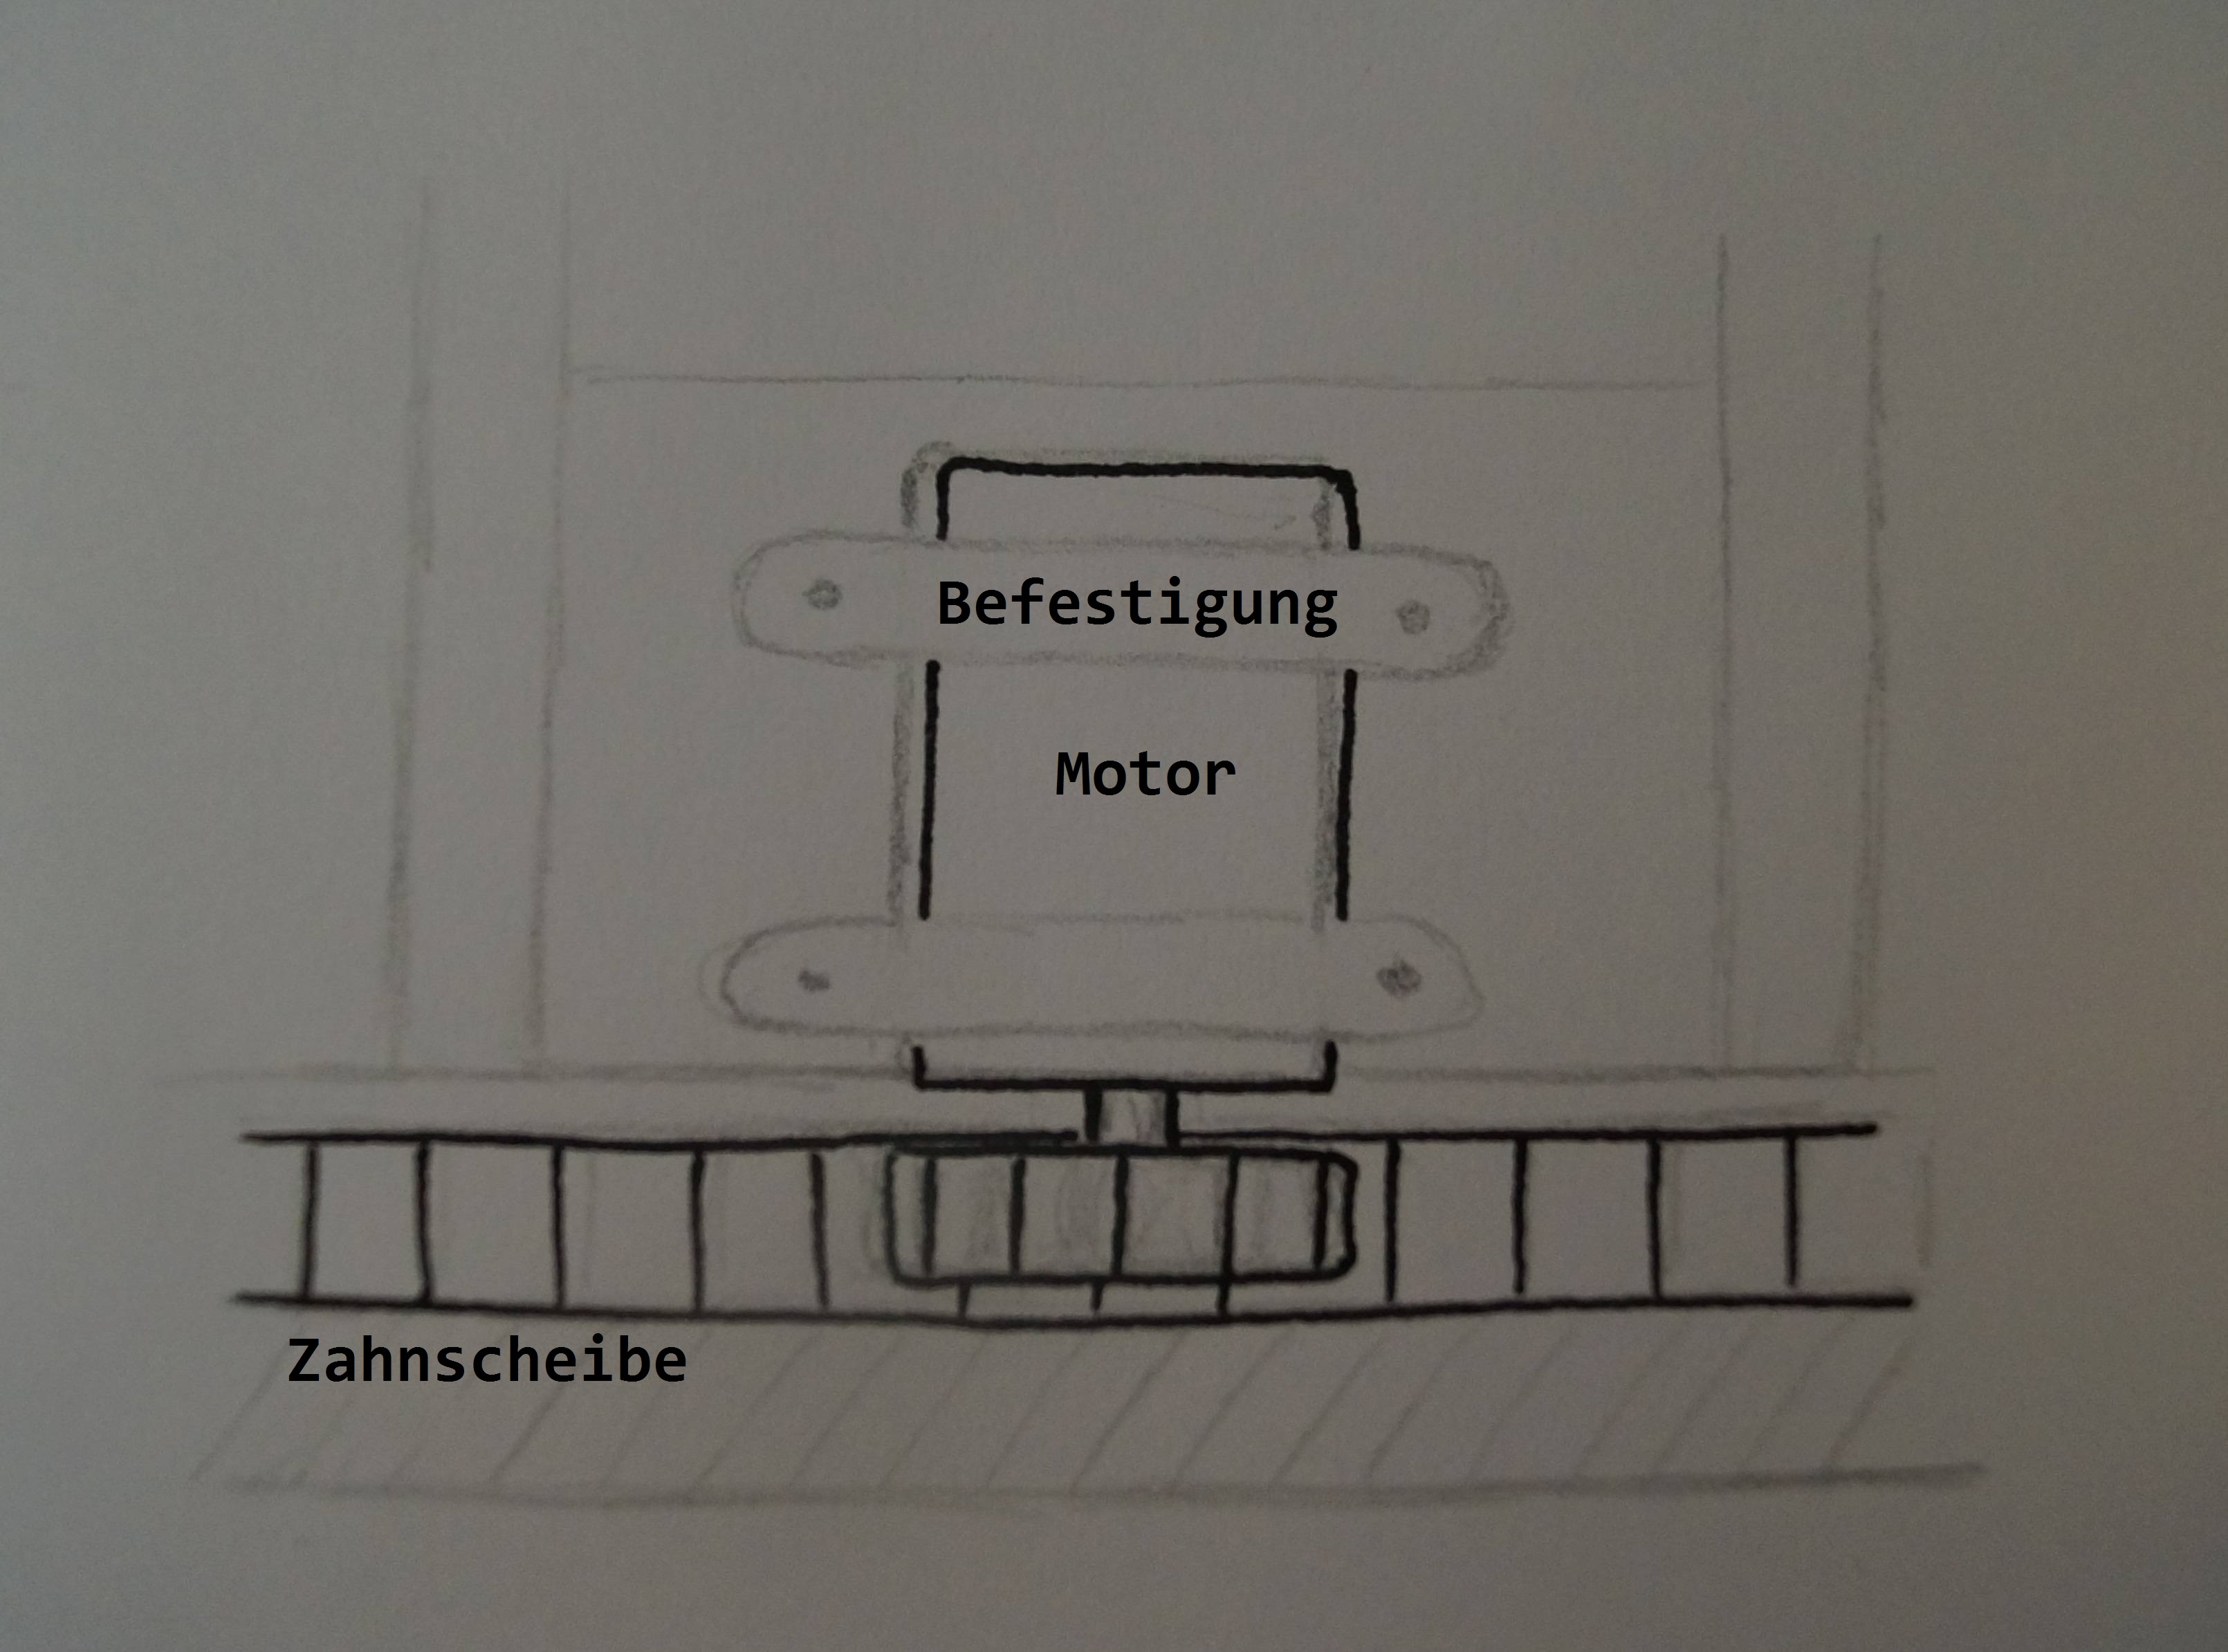
\includegraphics[scale=0.35]{../../fig/Ausrichtvorrichtung_Detail.jpg}
	\caption{Ausricht-Vorrichtung von der Seite}
	\label{fig:ausricht-vorrichtung-von-der-seite}
\end{figure}
Abbildung \ref{fig:ausricht-vorrichtung-von-der-seite} zeigt den Zahnradeingriff im Detail von der Seite.
